\section{Reachability, value fields, and flatness}
\label{sec:reachability-hjb}

Geodesics are not the only closed geometric description.  For the linear
fixed-speed model
\[
 \dot{\vect x}=\matr A\vect x+\matr B\vect u,
 \tag{30.1}
\]
consider fixed horizon \(T\), fixed endpoints, and minimum control energy
\(\int_0^T\vect u^{\mathsf T}\matr W_u\vect u\,dt\).  Define
\[
 \gls{sym:wc}=\int_0^T e^{\matr A\tau}\matr B\matr W_u^{-1}
 \matr B^{\mathsf T}e^{\matr A^{\mathsf T}\tau}\,d\tau,
 \quad
 \vect\delta=\vect x_B-e^{\matr A T}\vect x_A.
 \tag{30.2}
\]
If \(\matr W_c\succ0\), the exact solution is
\begin{align}
 J_u^\star&=\vect\delta^{\mathsf T}\matr W_c^{-1}\vect\delta,
 \tag{30.3}\\
 \vect u^\star(t)&=\matr W_u^{-1}\matr B^{\mathsf T}
 e^{\matr A^{\mathsf T}(T-t)}\matr W_c^{-1}\vect\delta.
 \tag{30.4}
\end{align}
The unit-energy reachable endpoints form
\(\vect\delta^{\mathsf T}\matr W_c^{-1}\vect\delta\leq1\).  A long axis is
easy to reach, a short axis expensive, and rotation exposes coupled dynamics.
This Gramian ellipsoid is neither the copper-loss ellipsoid nor the
instantaneous velocity ellipsoid.

\begin{figure}[tb]
\centering
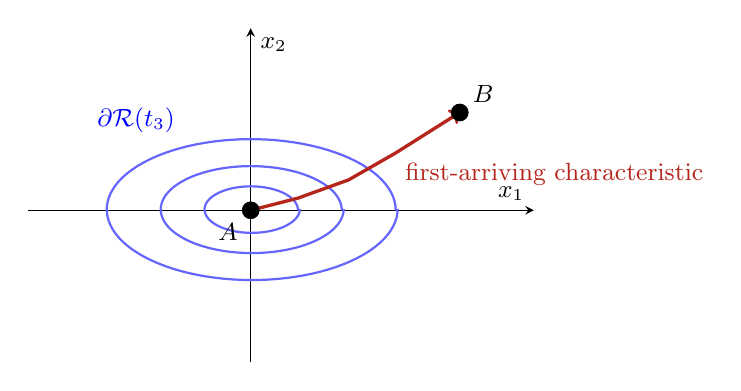
\begin{tikzpicture}[font=\small]
 \begin{axis}[width=.78\linewidth,height=.48\linewidth,axis equal image,
  axis lines=middle,xmin=-3.3,xmax=4.2,ymin=-2.25,ymax=2.7,ticks=none,xlabel={$x_1$},ylabel={$x_2$},clip=false]
  \foreach \a/\b/\c in {.7/.35/20,1.35/.65/35,2.15/1.05/55}{
   \addplot[blue!60,thick,domain=0:360,samples=100] ({.03*x/360+\a*cos(x)},{.02*x/360+\b*sin(x)});}
  \addplot[only marks,mark=*,black,mark size=3pt] coordinates {(0,0)(3.1,1.45)};
  \node[anchor=north east] at (axis cs:-.05,-.05) {$A$};
  \node[anchor=south west] at (axis cs:3.15,1.45) {$B$};
  \addplot[BrickRed,very thick,->] coordinates {(0,0)(.7,.18)(1.45,.45)(2.15,.85)(3.1,1.45)};
  \node[blue,anchor=south] at (axis cs:-1.7,1.0) {$\partial\mathcal R(t_3)$};
  \node[BrickRed,anchor=north west] at (axis cs:2.15,.85) {first-arriving characteristic};
 \end{axis}
\end{tikzpicture}
\caption{Reachability as an expanding wavefront.  Minimum time is the first
contact of the reachable set with the target; the optimal trajectory is a
characteristic of the arrival-time field.}
\label{fig:reachability-wavefront}
\end{figure}



The Gramian solution ignores hard voltage amplitude and path constraints.  It
is nevertheless an exact benchmark, a local design descriptor, and an
excellent warm start for constrained optimization.  Small eigenvalues of
\(\matr W_c\) identify dynamically weak directions; the condition number
measures reachability anisotropy over the declared horizon.

\subsection{Wavefront and Hamilton--Jacobi views}

Let \(\gls{sym:rset}\) contain all states reachable from \(A\) by time \(t\).
The minimum time to \(B\) is the first-contact time
\[
 t_{\min}(A,B)=\inf\{t:B\in\mathcal R(t)\}.
 \tag{30.5}
\]
Equivalently, let \(\gls{sym:value}\) be minimum remaining time to a target.
In regions where it is differentiable, dynamic programming gives
\[
 \boxed{\min_{\vect u\in\mathcal U}
 \left\{\nabla V^{\mathsf T}(\vect f+\matr B\vect u)+1\right\}=0.}
 \tag{30.6}
\]
For a drift-free Riemannian speed body, this reduces to an Eikonal equation;
with drift or a polyhedral converter it is the corresponding anisotropic HJB
equation.  Level sets \(V=c\) are equal-arrival-time wavefronts and optimal
paths are their characteristics.  This view avoids guessing a path: expand
the reachable-time wave and trace back the first-arriving characteristic.

Fast marching is exact only for an appropriate monotone Eikonal discretization
\parencite{sethian1996}; general drift and nonconvex state constraints may
require ordered upwind, fast sweeping, semi-Lagrangian, or value iteration
methods.  An embedded realization can store a coarse offline value map and
interpolate its descent direction, much like an MTPA/MTPV table, but memory
grows exponentially with state dimension.

\subsection{Differential flatness: useful, but not a metric}

For the fixed-speed electrical subsystem with nonsingular
\(\matr L_{\mathrm{diff}}\), choosing current itself as an output gives
\[
 \vect u=\matr L_{\mathrm{diff}}(\vect i)\dot{\vect i}
 +\vect r(\vect i,\omega_e).
 \tag{30.7}
\]
In this input-state sense the fully actuated electrical subsystem admits a
trivial flat parametrization: a differentiable current curve reconstructs the
required voltage algebraically.  That does not make every curve feasible or
optimal.  Voltage, current, torque, and thermal inequalities become constraints
on the output and its derivatives.  Polynomial or spline coefficients can
therefore reduce a trajectory search to finite dimension, consistent with the
flatness philosophy of \textcite{fliess1995}.

For the full electromechanical system the claim depends on outputs, load-torque
knowledge, position representation, and machine model; no global flatness is
asserted here.  The EESM adds a third electrical input and state, but saturation
and converter coupling remain.  Flatness parametrizes candidate curves;
Finsler geometry prices local travel; HJB evaluates globally optimal arrival;
MPC enforces constraints online.  They solve different parts of the problem.

\begin{table}[tb]
\centering
\caption{Dynamic methods classified by the physical question they simplify.}
\label{tab:dynamic-methods}
\begin{tabularx}{\linewidth}{@{}lXXX@{}}
\toprule
Method & Exact sweet spot & Hard constraints & Embedded implication\\
\midrule
Gramian & LTI, fixed horizon, quadratic input energy & not inherent & fixed matrix exponential/inverse\\
Analytic geodesic & smooth low-dimensional metric & boundary arcs separate & ODE integration, shooting\\
Polyhedral Finsler & exact converter facets & natural locally & switching/facet logic\\
Flat outputs & reconstructible states and inputs & coefficient inequalities & small spline program\\
Direct MPC & finite-horizon sampled model & explicit & iterative QP/NLP\\
Offline HJB & low-dimensional stationary dynamics & explicit in grid & LUT plus interpolation\\
Fast--slow reduction & separated time scales & reduced constraints & scalar scheduling plus fast inner law\\
\bottomrule
\end{tabularx}
\end{table}

